\documentclass[]{auvsi_doc}
\setkeys{auvsi_doc.cls}{
	AUVSITitle={Airframe Concept Description},
	AUVSILogoPath={./figs/logo.pdf}
}

% include extra packages, if needed

\begin{document}

\begin{AUVSITitlePage}
\begin{artifacttable}
\entry{AF-002, 0.1, 10-31-18, Initial Draft, Tyler Critchfield, Ryan Anderson}
\entry{AF-002, 0.2, 11-06-18, Revisions for Final Submission, Tyler Critchfield, Ryan Anderson}

% additional \entry{} commands for extra rows in the revision table, if needed
\end{artifacttable}
\end{AUVSITitlePage}

\section{Introduction}

This artifact describes our chosen airframe concept and how it relates to the Key Success Measures artifact.

\section{Concept Description}

We selected the modified Nimbus Pro for the Airframe subsystem. This airframe modifies a traditional twin propulsion fixed wing RC airframe (see Figure \ref{fig:nimbus}) that can be purchased off the shelf. The original RC airframe has a wing span of 1.95m, a wing area of 5700 cm$^2$, a fuselage length of 1.29m, a payload storage volume of about 8000 cm$^3$, and an empty weight of 1.9 kg. In this design, about two-thirds of the wings are able to be disconnected for easy storage and transport (see Figure \ref{fig:wing}). We could use this to our advantage and create new wing extensions to attach to the plane instead of the original wings. These wing extensions would likely have a longer span, but would be restricted to the existing design in root airfoil shape and root chord length. We would have freedom to adjust span, taper ratio, tip twist, and a tip airfoil if we so choose. We would model these design parameters in XFLR5 to determine the best wing extension design. The wing extensions would be made of foam and easily constructed using the foam cutter in EB 112.

The modular nature of these adjustments would make it easy to assemble and rebuild if necessary, especially if redundant parts are purchased and created. The lack of a modular, easily rebuild-able design was almost detrimental to last year's team when a crash shortly before the competition forced them to completely re-design their airframe. We hope to avoid this problem this year by implementing a modular design. To be successful, vision, controls, and UGV subsystem teams will need to prototype and test their designs often, but no one can truly test their designs without an airframe that flies. Having a modular wing design would still allow for fast rebuild, ensuring that other team members would not be wasting time waiting for the airframe to be rebuilt. In the case that a redesign is necessary, the other subsystem teams can use the off-the-shelf wings for the Nimbus Pro while waiting. Also, in the case that we find other design activities that take precedence over redesigning the wings, the original Nimbus Pro design will theoretically still work without modifications, albeit not as well. This provides flexibility in how we allocate our time.

\section{Key Success Measures}

This airframe concept was selected to optimize the achievement of the key success measures, which in turn will help us maximize our competition performance. First, we needed an airframe that could fly at a slower velocity. A slower velocity will increase maneuverability, making it easier for the autopilot to plan and execute a flight path that minimizes obstacles hit and improves waypoint proximity - two of our key success measures. In addition, a slower velocity will improve the image quality of our camera, which will theoretically increase the percentage of object characteristics identified. A slower velocity will also help airdrop accuracy. 

Second, we needed an airframe with sufficient storage capacity to carry the payload. Since this year's competition requires us to drop a UGV (Unmanned Ground Vehicle) in addition to a water bottle, sufficient fuselage volume is desirable. Payload storage capacity will prevent us from needing to mount the payload to the airframe exterior. Keeping the payload inside the airframe will prevent excess drag and allow the plane to fly at a slower velocity, assisting all of the key success measures already mentioned.

Third, the time to build the airframe was another measure we used in concept selection that indirectly affects all of the key success measures. If the airframe takes too long to build, it is difficult for us to test our other subsystems that are directly working on those key success measures (e.g. imaging subsystem needing to test identified characterisitcs).

\begin{figure}[h!]
	\centering
	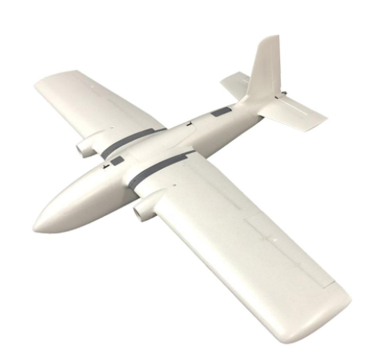
\includegraphics[scale=0.7]{figs/NimbusPro}
	\caption{The Nimbus Pro from My Fly Dream. Image taken from banggood.com.}
	\label{fig:nimbus}    
\end{figure}

\begin{figure}[h!]
	\centering
	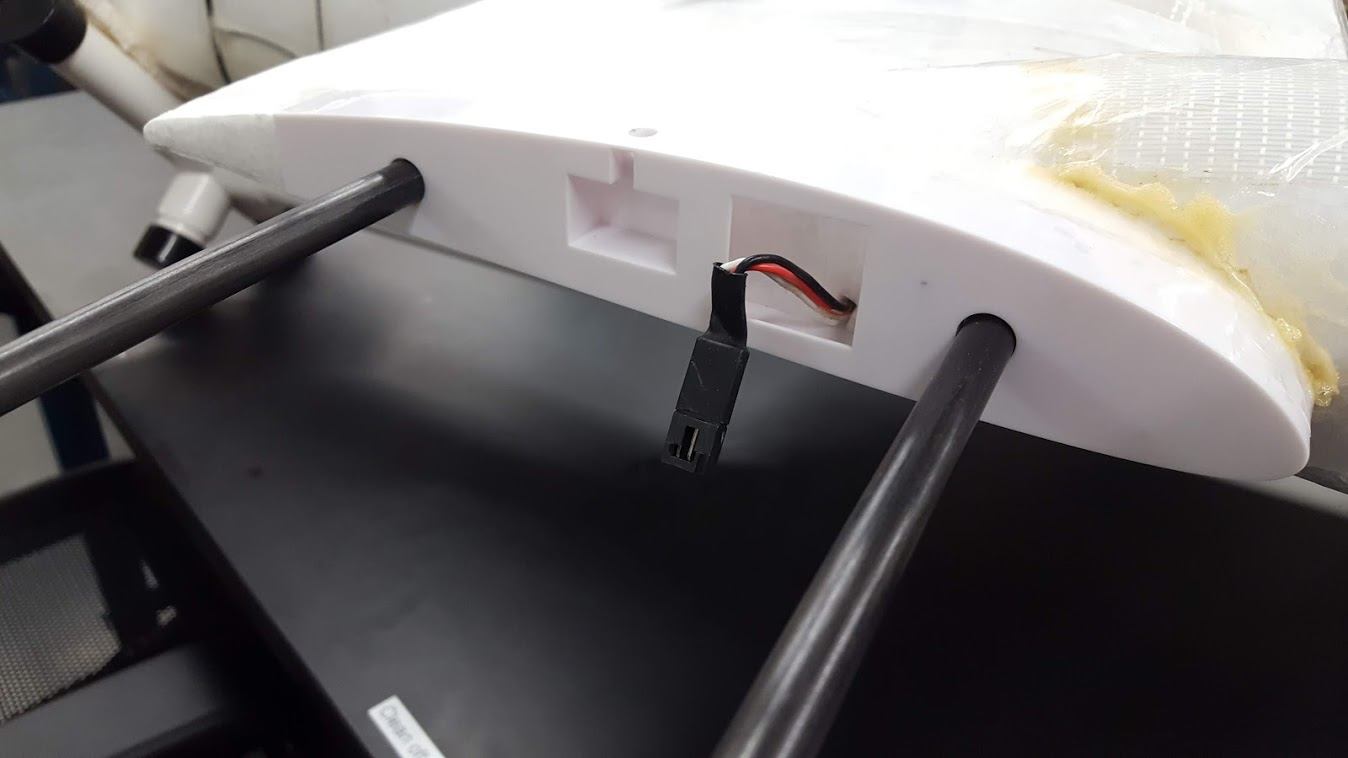
\includegraphics[width=.8\columnwidth]{figs/wing}
	\caption{This is where the wing disassembles and where we would attach our custom wings. This is a photo of My Twin Dream, but this concept is the same for the Nimbus Pro.}
	\label{fig:wing}    
\end{figure}

\section{Conclusion}

In short, the selected concept was chosen to optimize our key success measures. We are confident the Modified Nimbus Pro concept will help us maximize our performance in competition.


\end{document}